\documentclass[12pt,letterpaper]{article}

% just for the example
\usepackage{lipsum}
% Set margins to 1.5in
\usepackage[margin=1.5in]{geometry}

% for graphics
\usepackage{graphicx}
\graphicspath{{./figures/p2/}}

% for crimson text
\usepackage{crimson}
\usepackage[T1]{fontenc}

% setup parameter indentation
\setlength{\parindent}{0pt}
\setlength{\parskip}{6pt}

% for 1.15 spacing between text
\renewcommand{\baselinestretch}{1.15}

% For defining spacing between headers
\usepackage{titlesec}
% Level 1
\titleformat{\section}
  {\normalfont\fontsize{18}{0}\bfseries}{\thesection}{1em}{}
% Level 2
\titleformat{\subsection}
  {\normalfont\fontsize{14}{0}\bfseries}{\thesection}{1em}{}
% Level 3
\titleformat{\subsubsection}
  {\normalfont\fontsize{12}{0}\bfseries}{\thesection}{1em}{}
% Level 4
\titleformat{\paragraph}
  {\normalfont\fontsize{12}{0}\bfseries\itshape}{\theparagraph}{1em}{}
% Level 5
\titleformat{\subparagraph}
  {\normalfont\fontsize{12}{0}\itshape}{\theparagraph}{1em}{}
% Level 6
\makeatletter
\newcounter{subsubparagraph}[subparagraph]
\renewcommand\thesubsubparagraph{%
  \thesubparagraph.\@arabic\c@subsubparagraph}
\newcommand\subsubparagraph{%
  \@startsection{subsubparagraph}    % counter
    {6}                              % level
    {\parindent}                     % indent
    {12pt} % beforeskip
    {6pt}                           % afterskip
    {\normalfont\fontsize{12}{0}}}
\newcommand\l@subsubparagraph{\@dottedtocline{6}{10em}{5em}}
\newcommand{\subsubparagraphmark}[1]{}
\makeatother
\titlespacing*{\section}{0pt}{12pt}{6pt}
\titlespacing*{\subsection}{0pt}{12pt}{6pt}
\titlespacing*{\subsubsection}{0pt}{12pt}{6pt}
\titlespacing*{\paragraph}{0pt}{12pt}{6pt}
\titlespacing*{\subparagraph}{0pt}{12pt}{6pt}
\titlespacing*{\subsubparagraph}{0pt}{12pt}{6pt}

% Set caption to correct size and location
\usepackage[tableposition=top, figureposition=bottom, font=footnotesize, labelfont=bf]{caption}

% set page number location
\usepackage{fancyhdr}
\fancyhf{} % clear all header and footers
\renewcommand{\headrulewidth}{0pt} % remove the header rule
\rhead{\thepage}
\pagestyle{fancy}

% Overwrite Title
\makeatletter
\renewcommand{\maketitle}{\bgroup
   \begin{center}
   \textbf{{\fontsize{18pt}{20}\selectfont \@title}}\\
   \vspace{10pt}
   {\fontsize{12pt}{0}\selectfont \@author} 
   \end{center}
}
\makeatother

% Used for Tables and Figures
\usepackage{float}

% For using lists
\usepackage{enumitem}

% For using APA Citation format
\usepackage{apacite}

% Custom Quote
\newenvironment{myquote}[1]%
  {\list{}{\leftmargin=#1\rightmargin=#1}\item[]}%
  {\endlist}
  
% Create Abstract 
\renewenvironment{abstract}
{\vspace*{-.5in}\fontsize{12pt}{12}\begin{myquote}{.5in}
\noindent \par{\bfseries \abstractname.}}
{\medskip\noindent
\end{myquote}
}

\begin{document}

% Set Title, Author, and email
\title{Assignment P2}
\author{Snejana Shegheva \\ sshegheva3@gatech.edu}

\maketitle
\thispagestyle{fancy}

\begin{abstract}
 
\end{abstract}

\subsection*{Question 1. Georgia Tech - Online Registration}
The current process for which students have to register for the class at Georgia Tech is far from trivial as it requires a series of steps to be executed in a following order:

\begin{enumerate}
    \item Login to Buzzport with a multifactor authentication
    \item Location and click the \textit{Registration - Oscar} link 
    \item Click on the first item in the list \textit{Student Services and Financial Aid}
    \item Click \textit{Registration}
    \item Click \textit{Add or Drop Classes}
    \item From the Drop-down menu select the term for which you want to add a class
    \item Click on \textit{Advanced Search} tab at the bottom to be able to select subjects
    \item On the presented form select one or more \textit{Subjects}
    \item On the same form select \textit{Campus} - online
    \item Press \textit{Section Search}
    \item You are presented with a list of classes and their metadata. Find the class you are interested in and check the box to add the class
    \item Finally click \textit{Register}
\end{enumerate}

Registering for a class, therefore, is a complex undertaking, which is time-consuming and error prone in the areas of selecting the right subjects and desired term. A contra-intuitive requirement to select campus for an \textit{online} student adds another source for mistakes.
The registration interface can be re-designed by leveraging a great concept such as \textit{direct manipulation}. Using an analogy of physically visiting a department, and a classroom where the class we wish to enroll in would take place, we can re-design the current interface that gives user a sense of immersion\footnote{If your experience of physical enrollment differs, think of the example of signing up for drama or chess class with the blank paper hanging on the door inviting students to sign in.}. After logging in, the student navigates to the department of interest, for example, Computer Science, and lands on its home page. Here, the student is presented with available classes. Figure~\ref{fig::1} demonstrates a an imaginary list of courses offered in CS department \footnote{The departure from reality was due to lack of relevant image that portrays the idea nicely.} where user further narrows down to a course they are interested in. Clicking on the course section of the interface takes the student to the course summary

\begin{figure}[H]
\centering
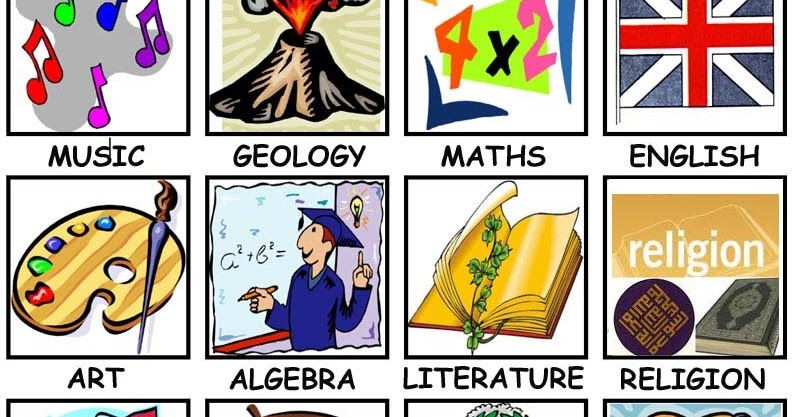
\includegraphics[width=3in,scale=.3]{figures/p2/school_subjects_modified.jpg}
\caption{Pictionary of School subjects. Image extracted from http://inglesmariapacheco.blogspot.com/2013/10/school-subjects.html}
\label{fig::1}
\end{figure}



\subsection*{Question 2 - Security System Panel}

\subsection*{Question 3 - Human perception feedback}

Auditory: seat belt is not buckled  
Visual: Light flash on the panel when signaling a turn 
Haptic: Pressing the car honk

Haptic: Vibrate the wheel if the turn the car is making is too sharp
Visual: Show on the panel when the distance to the nearby car crosses two seconds
Auditory: Speed points - very short beep at each one

Cold air into the face as the person is falling asleep.

\bibliographystyle{apacite} 
\bibliography{bibtemp}

\end{document}
